\subsection*{Differentialregning}
\begin{opgave}{Hastighed og postion}
	\begin{figure}[]
		\centering
		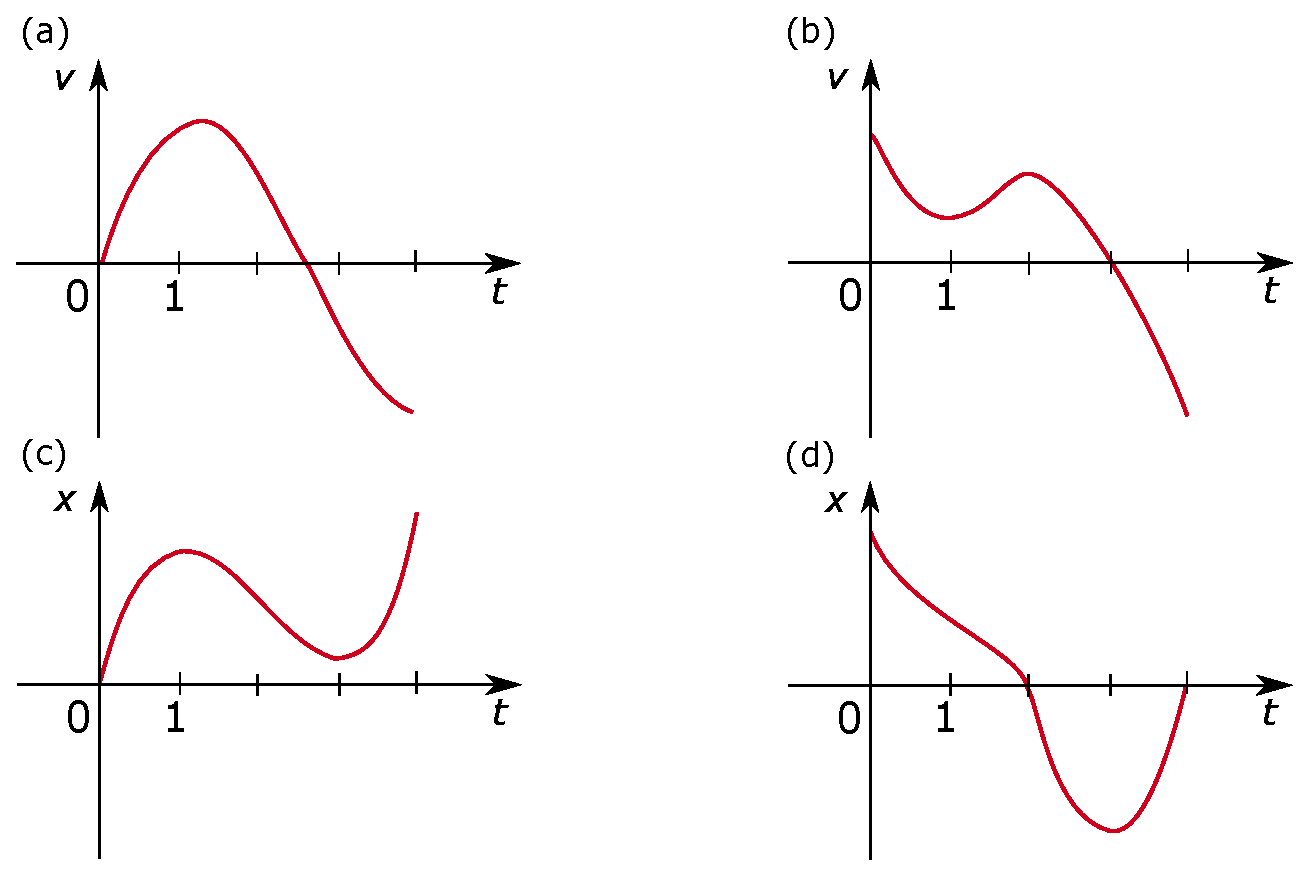
\includegraphics[width=0.47\textwidth]{Matematik/matfig/vx_grafer.eps}
		\caption{Hastighed og position som funktion af tiden.}
		\label{fig:vx_grafer_facit}
	\end{figure}
	\opg \Cref{fig:vx_grafer_facit} (a) og (b) viser hastigheden af to objekter som funktion af tiden i sekunder. Hvornår sætter de to objekter hastigheden op, og hvornår sætter de hastigheden ned? Forklar dit svar.
	
	De to objekter sætter hastigheden op når accelerationen er positiv, d.v.s. at hastighedsgrafen er stigende.
	For (a) er det inden toppunktet lidt efter $t=1$.
	For (b) stiger hastigheden imellem $t=1$ og $t=2$.
	\opg \Cref{fig:vx_grafer_facit} (c) og (d) viser positionen af to objekter $x$ som funktion af tiden i sekunder. Hvornår sætter de to objekter hastigheden op, og hvornår sætter de hastigheden ned? Forklar dit svar.
	
	De to objekter sætter hastigheden op når accelerationen er positiv, d.v.s. at krumningen er positiv. Her bruges smiley reglen.
	
	For (c) er krumningen negativ fra $t=0$ til $t=2$, og derefter positiv.
	For (d) er krumningen positiv over alt undtagen et lille stykke imellem $t=1$ og $t=2$.
\end{opgave}

\begin{opgave}[1]{Afledede og dobbeltafledede}
Find den afledede og dobbeltafledede med hensyn til $x$ for følgende funktioner:
\opg $f(x) = x^3$:
    \begin{align*}
        \dv{f}{x}&=3x^2, \\
        \dv[2]{f}{x}&=6x.
    \end{align*}
\opg $f(x) = x^2 + 4x$:
    \begin{align*}
        \dv{f}{x}&=2x+4,\\
        \dv[2]{f}{x}&=2.
    \end{align*}
\opg $f(x) = \dfrac{1}{x} + \dfrac{1}{x^2}$:
    \begin{align*}
        \dv{f}{x}&=-\frac{1}{x^2}-\frac{2}{x^3}, \\
        \dv[2]{f}{x}&=\frac{2}{x^3}+\frac{3}{x^4}.
    \end{align*}
\opg $f(x) = \cos(x)$:
    \begin{align*}
        \dv{f}{x}&=-\sin(x), \\
        \dv[2]{f}{x}&= -\cos(x).
    \end{align*}
\opg $f(x) = \ln(x)$:
    \begin{align*}
        \dv{f}{x}&=\frac{1}{x}, \\
        \dv[2]{f}{x}&=\frac{-1}{x^2}.
    \end{align*}

Til de sidste to delopgaver skal vi bruge produktregelen, der siger at den afledte af en funktion er:
%
\begin{align*}
    \dv{}{x}\big(f(x)g(x)\big)=\dv{f}{x}g(x)+f(x)\dv{g}{x}
\end{align*}
%
\opg $f(x) = x \sin(x)$:
    \begin{align*}
        \dv{f}{x}&=\sin(x)+x\cos(x), \\
        \dv[2]{f}{x}&=2\cos(x)-x\sin(x).
    \end{align*}
\opg $f(x) = \frac{1}{x} \ln(x)$:
    \begin{align*}
        \dv{f}{x}&=\frac{1}{x}\cdot \frac{1}{x}-\frac{1}{x^2}\cdot \ln(x)=\frac{1-\ln(x)}{x^2}, \\
        \dv[2]{f}{x}&=\frac{-1}{x^2}+\frac{2\ln(x)}{x^3}-\frac{1}{x^3}=\frac{2\ln(x)-x-1}{x^3}.
    \end{align*}
%
Her kunne man også have brugt kvotient regelen.
\end{opgave}

\begin{opgave}[2]{Sammensatte funktioner}
Skriv følgende udtryk som en sammensat funktion $f(g(x))$ (altså skal du identificere den indre funktion $g(x)$ og den ydre funktion $f(g)$). Beregn derefter $\dv*{f}{x}$.

Kædereglen siger: $\dv*{f}{x}=\dv*{f}{g} \cdot \dv*{g}{x}$.
\opg $f(x) = \sin (4x)\:,~~~g(x)=4x\:,~~~f(g)=\sin(g)\:,~~~\displaystyle\dv{f}{x}=4\cos(4x).$
\opg $f(x) = \sqrt{2x}\:,~~~g(x)=2x\:,~~~f(g)=\sqrt(g)\:,~~~\displaystyle\dv{f}{x}=\dfrac{1}{\sqrt{2x}}.$
\opg $f(x) = \sqrt{4x+5}\:,~~~g(x)=4x+5\:,~~~f(g)=\sqrt{g}\:,~~~\displaystyle\dv{f}{x}=\frac{2}{\sqrt{4x+5}}.$
\opg $f(x) = \sin(e^x)\:,~~~g(x)=e^x\:,~~~f(g)=\sin(g)\:,~~~\displaystyle\dv{f}{x}=e^x\cos(e^x).$
\opg $f(x) =  \ln \left( \cos x \right)\:,~~~g(x)=\cos(x)\:,~~~f(g)=\ln(g)\:,~~~\displaystyle\dv{f}{x}=\dfrac{-\sin(x)}{\cos(x)}=-\tan(x).$
\end{opgave}
%%
%%
\begin{opgave}[3]{Funktioner af flere variable - partiel differentiering}
	\opg $f(x,y,z) = x+y^2+z^3$:
	\begin{align*}
	\pdv{f}{x} = 1 \, , \quad
	\pdv{f}{y} = 2y \, , \quad
	\pdv{f}{z} = 3z^2 \, .
	\end{align*}
	\opg $f(x,y,z)=xy^2+ye^{-z}$:
	\begin{align*}
	\pdv{f}{x} = y^2 \, , \quad
	\pdv{f}{y} = 2xy+e^{-z} \, , \quad
	\pdv{f}{z} = -ye^{-z} \, .
	\end{align*}
	\opg $f(x,y,z)=ze^{xyz}$:
	\begin{align*}
	\pdv{f}{x} = yz^2e^{xyz} \, , \quad
	\pdv{f}{y} = xz^2e^{xyz} \, , \quad
	\pdv{f}{z} = e^{xyz}+xyze^{xyz} \, .
	\end{align*}
	\opg $f(x,y,z) = \dfrac{x-y+5z}{x+y+z}$:
	\begin{align*}
	\pdv{f}{x} = \frac{2(y-2z)}{(x+y+z)^2} \, , \quad
	\pdv{f}{y} = -\frac{2(x+3z)}{(x+y+z)^2} \, , \quad
	\pdv{f}{z} = \frac{4x+6y}{(x+y+z)^2} \, .
	\end{align*}
\end{opgave}
%%